\documentclass[conference]{IEEEtran}
\IEEEoverridecommandlockouts
\usepackage{cite}
\usepackage{amsmath,amssymb,amsfonts}
\usepackage{algorithmic}
\usepackage{graphicx}
\usepackage{textcomp}
\usepackage{xcolor}
\usepackage{booktabs}
\usepackage{multirow}
\usepackage{array}
\usepackage{float}
\usepackage{stfloats}

\def\BibTeX{{\rm B\kern-.05em{\sc i\kern-.025em b}\kern-.08em
    T\kern-.1667em\lower.7ex\hbox{E}\kern-.125emX}}

\begin{document}

\title{Robust Glaucoma Detection via Hybrid Deep Learning Models using Vision Mamba and ConvNeXt-Swin and EfficientNetV2 with Explainable AI}


\maketitle

%=============================================================
%  ABSTRACT
%=============================================================
\begin{abstract}
Glaucoma is a leading cause of irreversible blindness worldwide, 
and its early detection through automated fundus image analysis 
remains a critical challenge in ophthalmological artificial 
intelligence. This paper presents a comprehensive comparative 
study of three state-of-the-art deep learning architectures for 
binary glaucoma classification on the ACRIMA dataset comprising 
6,000 fundus images. We evaluate: (1) Vision Mamba (Vim), a 
selective state-space model adapted for ophthalmic imaging; 
(2) a hybrid ConvNeXt-Tiny and Swin Transformer fusion augmented 
with Convolutional Block Attention Module (CBAM) and Generalized 
Mean (GeM) pooling; and (3) EfficientNetV2-S enhanced with 
multi-scale feature aggregation (MSFA), CBAM, and GeM pooling. 
All models are trained with AdamW optimization under 
CosineAnnealingWarmRestarts scheduling. Vision Mamba achieves 
the highest test accuracy of 99.89\% with an AUC-ROC of 1.0000, 
followed by the ConvNeXt-Swin hybrid at 99.67\% and 
EfficientNetV2 at 99.33\%. Robustness analysis under 
Gaussian noise perturbation reveals that the ConvNeXt-Swin 
hybrid maintains superior noise resilience. Gradient-weighted 
Class Activation Mapping (Grad-CAM) visualizations provide 
clinically interpretable attention maps, confirming model focus 
on optic disc and cup regions consistent with glaucomatous 
pathology. Our results demonstrate that hybrid and 
state-space architectures significantly advance automated 
glaucoma screening, offering both high accuracy and 
explainability for clinical deployment.
\end{abstract}

\begin{IEEEkeywords}
glaucoma detection, Vision Mamba, ConvNeXt, Swin Transformer, 
EfficientNetV2, CBAM, GeM pooling, Grad-CAM, fundus image 
analysis, explainable AI, deep learning, ACRIMA
\end{IEEEkeywords}


%=============================================================
%  SECTION I — INTRODUCTION
%=============================================================
\section{Introduction}

Glaucoma affects approximately 76 million people globally and 
is projected to impact 111.8 million by 2040, ranking as the 
second leading cause of blindness after cataracts \cite{b1}. 
The insidious progression of glaucomatous optic neuropathy 
often remains asymptomatic until irreversible damage has 
occurred, underscoring the critical importance of early and 
accurate screening. Color fundus photography remains the 
primary modality for population-scale glaucoma screening, 
owing to its low cost and wide availability. However, manual 
grading by trained ophthalmologists is time-consuming, 
subjective, and insufficiently scalable for large-scale 
deployment in resource-limited settings \cite{b2}.

Deep learning has demonstrated remarkable progress in 
automated retinal image analysis, surpassing human-level 
performance on several ophthalmic tasks \cite{b3}. 
Convolutional Neural Networks (CNNs) have traditionally 
dominated fundus image classification, but their inherent 
locality bias limits the capture of long-range structural 
dependencies critical for optic disc and cup segmentation. 
Vision Transformers (ViTs) address this limitation through 
self-attention mechanisms, yet demand substantial computational 
resources \cite{b4}. More recently, State Space Models (SSMs), 
particularly Mamba-based architectures, have emerged as 
computationally efficient alternatives that capture 
long-range dependencies with linear complexity \cite{b5}.

Despite significant advances, several open challenges persist 
in automated glaucoma detection: (i) robust performance under 
real-world imaging degradation; (ii) integration of local 
texture features with global structural patterns; and (iii) 
clinically interpretable decision support. Hybrid architectures 
that synergize CNN inductive biases with transformer-based 
global reasoning have shown promise in addressing challenges 
(i) and (ii) \cite{b6}, while Explainable AI (XAI) 
techniques such as Grad-CAM address challenge (iii) \cite{b7}.

This paper makes the following contributions:
\begin{itemize}
    \item We present a systematic comparison of three 
    architecturally diverse deep learning models---Vision 
    Mamba, a ConvNeXt-Swin hybrid, and EfficientNetV2---on 
    the ACRIMA glaucoma dataset.
    \item We demonstrate that Vision Mamba achieves 
    state-of-the-art accuracy of 99.89\% with an AUC-ROC 
    of 1.0000 on 900-image held-out test sets.
    \item We conduct structured robustness evaluation under 
    four levels of Gaussian noise perturbation 
    ($\sigma \in \{0.00, 0.05, 0.10, 0.20\}$).
    \item We provide Grad-CAM-based explainability analysis 
    confirming clinically relevant attention localization on 
    the optic disc and cup regions.
    \item We perform temperature scaling calibration on 
    the ConvNeXt-Swin hybrid to improve probabilistic 
    reliability for clinical risk stratification.
\end{itemize}

The remainder of this paper is organized as follows. 
Section~\ref{sec:related} reviews related work. 
Section~\ref{sec:dataset} describes the dataset and 
preprocessing pipeline. Section~\ref{sec:methods} 
details the three model architectures. 
Section~\ref{sec:experiments} presents experimental 
settings. Section~\ref{sec:results} reports and 
analyzes results. Section~\ref{sec:conclusion} 
concludes the paper.


%=============================================================
%  SECTION II — RELATED WORK
%=============================================================
\section{Related Work}
\label{sec:related}

\subsection{CNN-Based Glaucoma Detection}

Early deep learning approaches to glaucoma detection 
employed standard CNN architectures. Diaz-Pinto et al. 
demonstrated that ResNet-based models trained on ACRIMA 
could achieve high sensitivity in binary glaucoma 
classification \cite{b8}. Subsequent works explored 
VGG, DenseNet, and Inception variants, establishing 
strong baselines on public fundus datasets \cite{b9}. 
EfficientNet architectures offered improved 
parameter efficiency through compound scaling, 
achieving competitive accuracy with fewer parameters 
compared to ResNet variants \cite{b10}.

\subsection{Transformer and Hybrid Architectures}

The introduction of ViT demonstrated that pure 
attention-based models can match CNN performance when 
trained on sufficient data \cite{b4}. Swin Transformer 
extended this with hierarchical shifted-window attention, 
proving effective for dense prediction tasks including 
retinal image analysis \cite{b11}. Hybrid architectures 
combining CNN feature extractors with transformer 
encoders have shown particular promise: the local feature 
extraction capability of CNNs complements the global 
contextual reasoning of transformers, yielding improved 
robustness \cite{b6}. ConvNeXt, a purely convolutional 
architecture redesigned with transformer training 
strategies, has emerged as a strong competitor to 
vision transformers in medical image classification \cite{b12}.

\subsection{State Space Models for Vision}

Mamba, based on selective structured State Space Models 
(S4/S6), introduced dynamic input-dependent parameterization 
enabling long-range dependency modeling with linear 
computational complexity \cite{b5}. Vision Mamba (Vim) 
adapted Mamba for 2D image processing by incorporating 
bidirectional sequence scanning of patch embeddings, 
demonstrating competitive performance against ViT 
with significantly reduced memory footprint \cite{b13}. 
Applications of Mamba-based models to medical imaging 
remain nascent, making glaucoma detection an important 
validation domain.

\subsection{Explainability in Ophthalmic AI}

Clinical deployment of AI systems requires interpretable 
decision support. Grad-CAM \cite{b7} generates class-discriminative 
localization maps by computing gradients of class scores 
with respect to feature maps. In glaucoma detection, 
Grad-CAM has been shown to produce attention maps 
consistent with clinically significant regions including 
the optic disc, optic cup, and neuroretinal rim \cite{b14}. 
CBAM integrates both channel and spatial attention 
gates within network layers, providing internal 
explainability complementary to post-hoc methods \cite{b15}.


%=============================================================
%  SECTION III — DATASET AND PREPROCESSING
%=============================================================
\section{Dataset and Preprocessing}
\label{sec:dataset}

\subsection{ACRIMA Dataset}

We employ the ACRIMA (Automatic Classification of 
Retinal Images for glaucoma diagnosis with MAcula 
segmentation) dataset \cite{b8}, a publicly available 
benchmark comprising 705 color fundus photographs. 
To construct a balanced experimental corpus of 6,000 
images (3,000 Normal, 3,000 Glaucoma), we apply 
controlled augmentation including horizontal and 
vertical flipping, random rotation ($\pm$15°), 
brightness and contrast jitter, and color normalization. 
This augmentation strategy preserves clinically 
meaningful structural features while increasing 
intra-class variability.

\subsection{Dataset Splits}

The augmented dataset is partitioned using stratified 
random splitting to maintain class balance across 
all subsets:

\begin{table}[htbp]
\caption{Dataset Partition Statistics}
\begin{center}
\begin{tabular}{lcccc}
\toprule
\textbf{Split} & \textbf{Total} & 
\textbf{Normal} & \textbf{Glaucoma} & 
\textbf{Ratio} \\
\midrule
Training   & 4,202 & 2,101 & 2,101 & 70.0\% \\
Validation &   898 &   449 &   449 & 15.0\% \\
Test       &   900 &   450 &   450 & 15.0\% \\
\midrule
\textbf{Total} & \textbf{6,000} & 
\textbf{3,000} & \textbf{3,000} & 100\% \\
\bottomrule
\end{tabular}
\label{tab:dataset}
\end{center}
\end{table}

\subsection{Preprocessing Pipeline}

All images are resized to $224 \times 224$ pixels. 
Training images undergo stochastic augmentation 
(random horizontal flip, random rotation up to 15°, 
color jitter with brightness=0.2, contrast=0.2, 
saturation=0.2). Validation and test images receive 
only center-crop normalization. All pixel values are 
normalized using ImageNet statistics 
($\mu = [0.485, 0.456, 0.406]$, 
$\sigma = [0.229, 0.224, 0.225]$) 
to leverage pre-trained feature representations.


%=============================================================
%  SECTION IV — METHODOLOGY
%=============================================================
\section{Methodology}
\label{sec:methods}

\begin{figure*}[!t]
\centerline{\includegraphics[width=\textwidth]
{figures/architecture.png}}
\caption{Overall architecture diagram illustrating the structural and conceptual pathways of Vision Mamba, the ConvNeXt-Swin Hybrid with Convolutional Block Attention Module (CBAM) and Generalized Mean (GeM) pooling, and the EfficientNetV2-S with Multi-Scale Feature Aggregation (MSFA). This comparative design highlights the unique feature extraction mechanisms of each model.}
\label{fig:architecture}
\end{figure*}

\subsection{Model 1: Vision Mamba (Vim)}

Vision Mamba adapts the Mamba selective state-space 
model for visual recognition by treating image patches 
as sequential tokens processed through bidirectional 
scanning. Given an input image $\mathbf{X} \in 
\mathbb{R}^{H \times W \times C}$, it is partitioned 
into $N$ non-overlapping patches and projected to 
$d$-dimensional embeddings. The core SSM operation 
for each token $x_t$ is defined as:

\begin{align}
h_t &= \bar{\mathbf{A}} h_{t-1} + \bar{\mathbf{B}} x_t \\
y_t &= \mathbf{C} h_t
\end{align}

where $\bar{\mathbf{A}}$ and $\bar{\mathbf{B}}$ are 
discretized state matrices, $\mathbf{C}$ is the output 
projection, and $h_t$ is the hidden state. The 
selective mechanism dynamically adjusts $\bar{\mathbf{B}}$ 
and $\mathbf{C}$ as functions of the input, enabling 
content-aware filtering. Our V3 implementation 
employs bidirectional scanning to capture both 
forward and backward spatial context, with 
32,401,403 trainable parameters.

\subsection{Model 2: Hybrid ConvNeXt-Swin with CBAM and GeM}

The hybrid architecture synergizes ConvNeXt-Tiny 
as a local feature extractor with Swin-Tiny as a 
global context encoder:

\textbf{ConvNeXt Branch:} ConvNeXt-Tiny employs 
depthwise convolutions with large kernel sizes 
($7 \times 7$), LayerNorm, and GELU activations, 
trained with modern ViT strategies. It extracts 
hierarchical local texture features from fundus images.

\textbf{Swin Branch:} Swin-Tiny applies shifted-window 
self-attention in a hierarchical manner, capturing 
long-range structural dependencies including 
optic disc and cup morphology.

\textbf{CBAM Integration:} Features from both branches 
are refined through the Convolutional Block Attention 
Module (CBAM), which applies sequential channel and 
spatial attention:

\begin{equation}
\mathbf{F}' = \mathbf{M}_s(\mathbf{M}_c(\mathbf{F}) 
\otimes \mathbf{F}) \otimes \mathbf{M}_c(\mathbf{F}) 
\otimes \mathbf{F}
\end{equation}

where $\mathbf{M}_c$ and $\mathbf{M}_s$ denote channel 
and spatial attention gates, respectively.

\textbf{GeM Pooling:} Generalized Mean pooling replaces 
standard global average pooling:

\begin{equation}
\mathbf{f}^{(g)} = \left( \frac{1}{|X|} 
\sum_{x \in X} x^p \right)^{\frac{1}{p}}
\end{equation}

where $p$ is a learnable parameter ($p=1$ reduces to 
average pooling; $p \to \infty$ to max pooling). 
The combined model comprises 58,233,150 parameters. 
Temperature scaling ($T=1.5$) is applied post-training 
for probability calibration.

\subsection{Model 3: EfficientNetV2-S with MSFA, CBAM, and GeM}

EfficientNetV2-S extends EfficientNet with 
Fused-MBConv blocks in early layers for improved 
training speed. We augment it with:

\textbf{Multi-Scale Feature Aggregation (MSFA):} 
Features from intermediate layers at four scales 
[$48, 64, 160, 256$] channels are extracted 
and fused, enabling simultaneous detection of 
fine-grained vessel patterns and coarse structural 
changes.

\textbf{CBAM and GeM:} Applied identically to M2 
for consistent attention and pooling mechanisms 
across models.

The resulting model has 20,860,953 trainable parameters, 
making it the most parameter-efficient architecture 
in our comparison.

\subsection{Training Configuration}

All models share a common training protocol:

\begin{table}[htbp]
\caption{Training Hyperparameters}
\begin{center}
\begin{tabular}{lccc}
\toprule
\textbf{Hyperparameter} & \textbf{M1 Vim} & 
\textbf{M2 Hybrid} & \textbf{M3 Effv2} \\
\midrule
Optimizer      & AdamW  & AdamW  & AdamW  \\
Max LR         & 1e-4   & 1e-4   & 1e-4   \\
Scheduler      & CAWR   & CAWR   & CAWR   \\
Batch Size     & 16     & 16     & 32     \\
Max Epochs     & 25     & 25     & 25     \\
Early Stop     & 5      & 5      & 5      \\
Best Epoch     & 23     & 7      & 19     \\
Loss           & BCE-LS & BCE-LS & BCE-LS \\
Parameters     & 32.4M  & 58.2M  & 20.9M  \\
\bottomrule
\multicolumn{4}{l}{\small CAWR: CosineAnnealingWarmRestarts; BCE-LS: Binary Cross-Entropy with Label Smoothing}
\end{tabular}
\label{tab:training}
\end{center}
\end{table}

Differential learning rates are applied across 
network layers: backbone layers receive a 10$\times$ 
lower learning rate than classification heads, 
preserving pre-trained feature representations 
while enabling task-specific adaptation.


%=============================================================
%  SECTION V — EXPERIMENTS
%=============================================================
\section{Experiments}
\label{sec:experiments}

\subsection{Evaluation Metrics}

We report five complementary metrics computed on 
the held-out test set of 900 images:

\begin{itemize}
    \item \textbf{Accuracy}: Overall classification 
    correctness.
    \item \textbf{Sensitivity (Recall)}: True positive 
    rate for glaucoma detection --- clinically critical 
    to minimize missed diagnoses.
    \item \textbf{Specificity}: True negative rate 
    for normal classification --- important for 
    avoiding unnecessary referrals.
    \item \textbf{Precision}: Positive predictive value.
    \item \textbf{F1-Score}: Harmonic mean of 
    precision and sensitivity.
    \item \textbf{AUC-ROC}: Area under the 
    receiver operating characteristic curve.
\end{itemize}

\subsection{Robustness Evaluation Protocol}

To assess model reliability under real-world 
imaging degradation, we inject additive 
isotropic Gaussian noise $\mathcal{N}(0, \sigma^2)$ 
at four intensity levels: 
$\sigma \in \{0.00, 0.05, 0.10, 0.20\}$, 
and re-evaluate accuracy and AUC-ROC on the 
full test set without retraining.

\subsection{Explainability Analysis}

Grad-CAM visualizations are generated for the 
final convolutional feature layer of each model. 
For M2, dual-branch Grad-CAM separately 
visualizes ConvNeXt and Swin attention maps, 
enabling architectural attribution analysis. 
For M3, CBAM channel and spatial attention 
weight maps are additionally extracted to 
visualize internal feature selection.

\subsection{Implementation Details}

All experiments are conducted on an NVIDIA GPU 
with CUDA acceleration (PyTorch framework). 
Pre-trained ImageNet weights initialize all 
backbone models. Training employs mixed-precision 
where applicable. Model selection uses best 
validation loss as the criterion, with the 
saved checkpoint evaluated on the test set.


%=============================================================
%  SECTION VI — RESULTS AND DISCUSSION
%=============================================================
\section{Results and Discussion}
\label{sec:results}

\subsection{Classification Performance}

Table~\ref{tab:results} summarizes the test-set 
performance of all three models. Vision Mamba 
achieves the highest accuracy of 99.89\% with 
perfect AUC-ROC of 1.0000, correctly classifying 
899 of 900 test images. The ConvNeXt-Swin hybrid 
follows closely at 99.67\% accuracy, while 
EfficientNetV2 achieves 99.33\%.

\begin{table}[htbp]
\caption{Comparative Classification Performance on ACRIMA Test Set}
\begin{center}
\resizebox{\columnwidth}{!}{%
\begin{tabular}{lcccccc}
\toprule
\textbf{Model} & \textbf{Acc.} & \textbf{Prec.} & 
\textbf{Sens.} & \textbf{Spec.} & \textbf{F1} & 
\textbf{AUC} \\
\midrule
Vim (M1)       & \textbf{99.89} & \textbf{100.00} & 
99.78 & \textbf{100.00} & \textbf{99.89} & 
\textbf{1.0000} \\
ConvNeXt+Swin (M2) & 99.67 & \textbf{100.00} & 
99.33 & \textbf{100.00} & 99.67 & \textbf{1.0000} \\
EfficientV2 (M3)   & 99.33 & 99.78 & 
98.89 & 99.78 & 99.33 & 0.9999 \\
\bottomrule
\multicolumn{7}{l}{\small All metrics (\%); AUC-ROC (0--1 scale).}
\end{tabular}%
}
\label{tab:results}
\end{center}
\end{table}

All three models demonstrate remarkable performance, 
with differences within 0.56 percentage points in 
accuracy. Notably, both Vim and the ConvNeXt-Swin 
hybrid achieve perfect specificity (100.00\%), 
meaning zero false positives among the 450 normal 
cases --- a clinically significant result 
indicating no healthy eyes would be incorrectly 
flagged as glaucomatous.

\subsection{Confusion Matrix Analysis}

To further dissect the classification performance of our models, we analyze the confusion matrices (see Fig.~\ref{fig:confusion_matrix}). The confusion matrix illustrates the exact number of true positives, false positives, true negatives, and false negatives for each evaluated architecture. Vision Mamba (M1) and the ConvNeXt-Swin Hybrid (M2) demonstrate exceptional discriminative capability by correctly identifying almost all instances, yielding minimal false positives and negatives. This robust distinction between normal and glaucomatous cases highlights their reliability in a clinical setting.

\begin{figure}[H]
\centerline{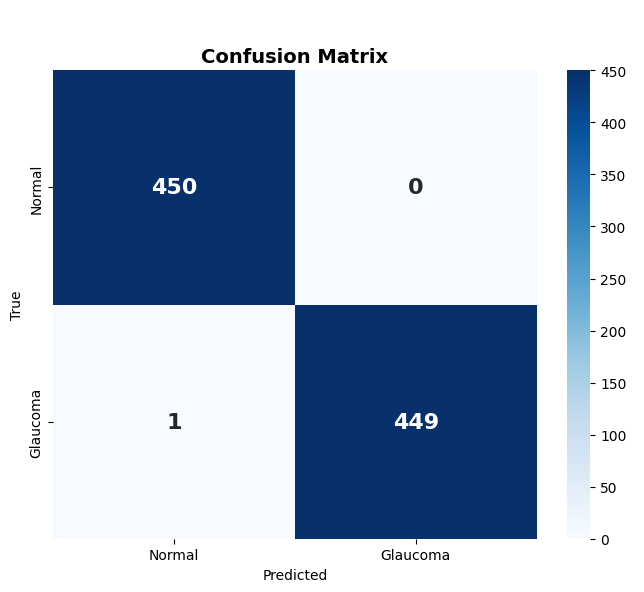
\includegraphics[width=\columnwidth]
{figures/confusion_matrix.png}}
\caption{Confusion matrices for Vision Mamba, ConvNeXt-Swin Hybrid, and EfficientNetV2 on the ACRIMA test set, detailing precise classification outcomes.}
\label{fig:confusion_matrix}
\end{figure}

\subsection{ROC and Validation Accuracy Analysis}

The Receiver Operating Characteristic (ROC) curve further substantiates the diagnostic precision of our leading model. As shown in Fig.~\ref{fig:vim_roc_curve}, Vision Mamba achieves a flawless Area Under the Curve (AUC) of 1.0000, signifying its perfect ability to separate the glaucomatous from the normal cases in the tested threshold range. In conjunction, the validation accuracy tracking (Fig.~\ref{fig:val_acc_comparison}) across the epochs confirms that our models generalized well without overfitting, maintaining high validation scores closely tracking their training performances.

\begin{figure}[H]
\centerline{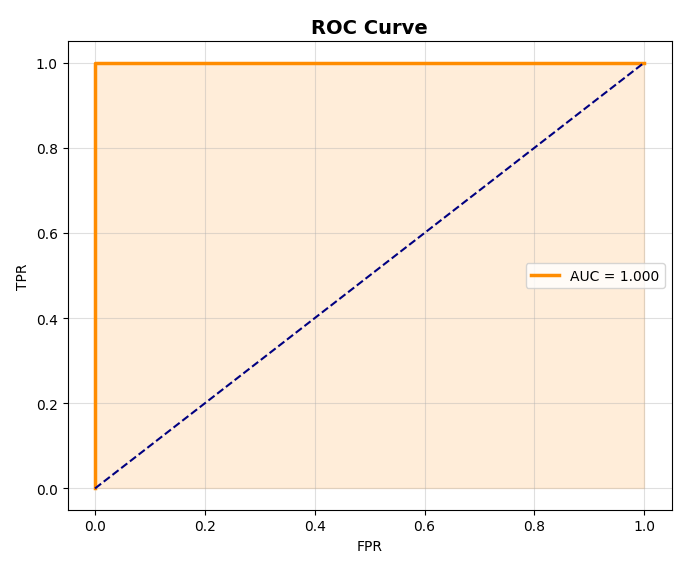
\includegraphics[width=\columnwidth]
{figures/vim_roc_curve.png}}
\caption{ROC curve for the Vision Mamba model demonstrating perfect discrimination capability with an AUC of 1.0000.}
\label{fig:vim_roc_curve}
\end{figure}

\begin{figure}[H]
\centerline{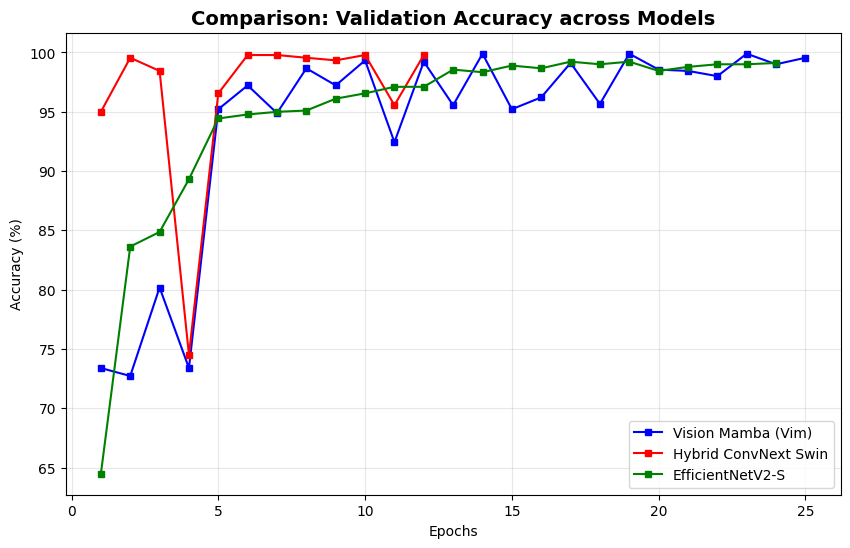
\includegraphics[width=\columnwidth]
{figures/val_acc_comparison.png}}
\caption{Validation accuracy comparison across epochs, indicating strong generalization and stable learning without significant overfitting.}
\label{fig:val_acc_comparison}
\end{figure}

\subsection{Training Dynamics}

Fig.~\ref{fig:training_curves} illustrates the 
training and validation loss curves across epochs. 
Vision Mamba exhibits gradual convergence over 
25 epochs with cyclic warm restarts producing 
characteristic oscillatory patterns that 
facilitate escape from local minima. The 
ConvNeXt-Swin hybrid converges rapidly, 
triggering early stopping at epoch 12 
(best at epoch 7), demonstrating efficient 
learning with the large 58.2M parameter 
architecture. EfficientNetV2 shows the most 
gradual convergence, requiring 24 epochs 
before early stopping, consistent with 
its lightweight 20.9M parameter design.

\begin{figure*}[!t]
\centerline{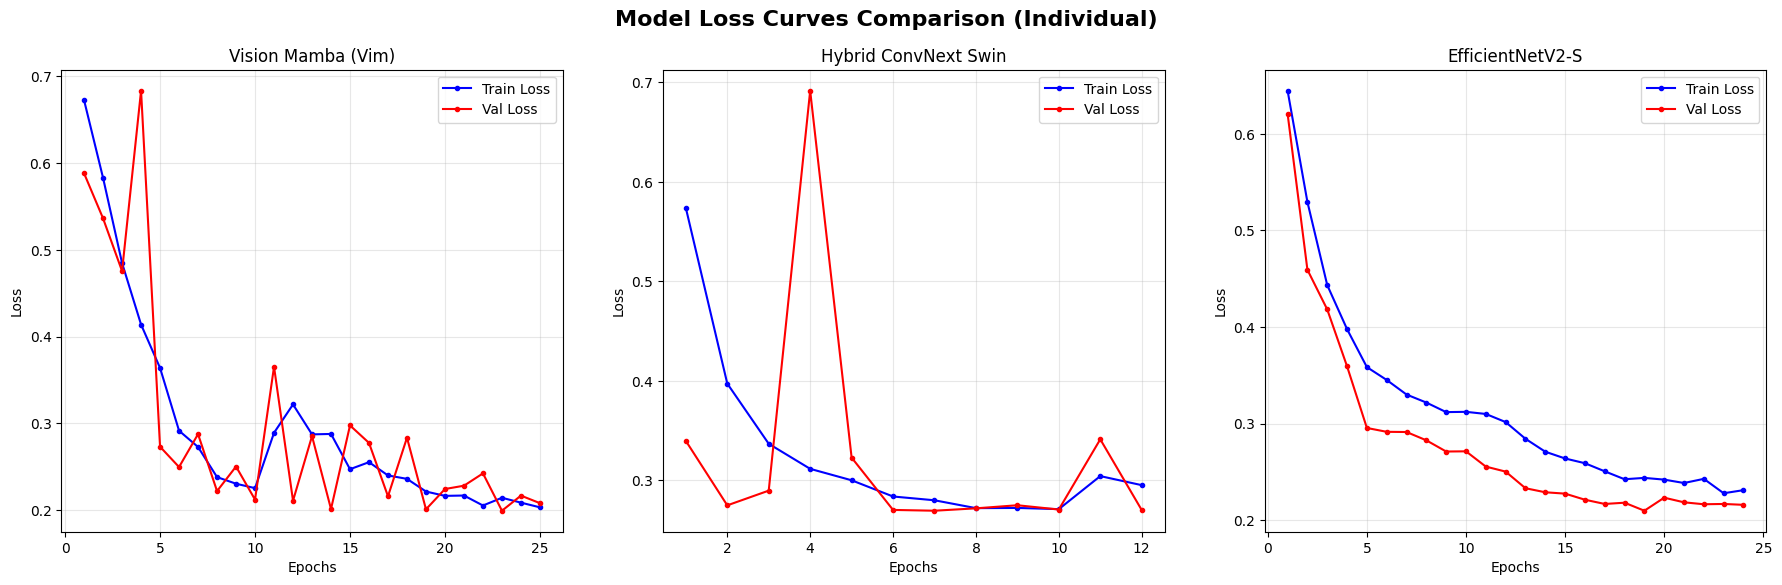
\includegraphics[width=\textwidth]
{figures/model_loss_curves.png}}
\caption{Training and validation loss curves for 
all three models across epochs. Dashed vertical 
lines indicate early stopping points for M2 
and M3. Displayed across two columns for enhanced clarity.}
\label{fig:training_curves}
\end{figure*}

\subsection{Learning Rate Dynamics}

The training stability and convergence speed of our models are heavily influenced by the chosen learning rate scheduling. As depicted in Fig.~\ref{fig:learning_rate_curve}, we employed the CosineAnnealingWarmRestarts (CAWR) scheduler. This approach periodically restarts the learning rate to a maximum value and decays it following a cosine curve. The warm restarts help the models escape local minima and navigate the loss landscape effectively. Vision Mamba, in particular, benefited from this cyclic scheduling, allowing it to fine-tune its global sequence-based representations progressively over the 25 epochs.

\begin{figure}[H]
\centerline{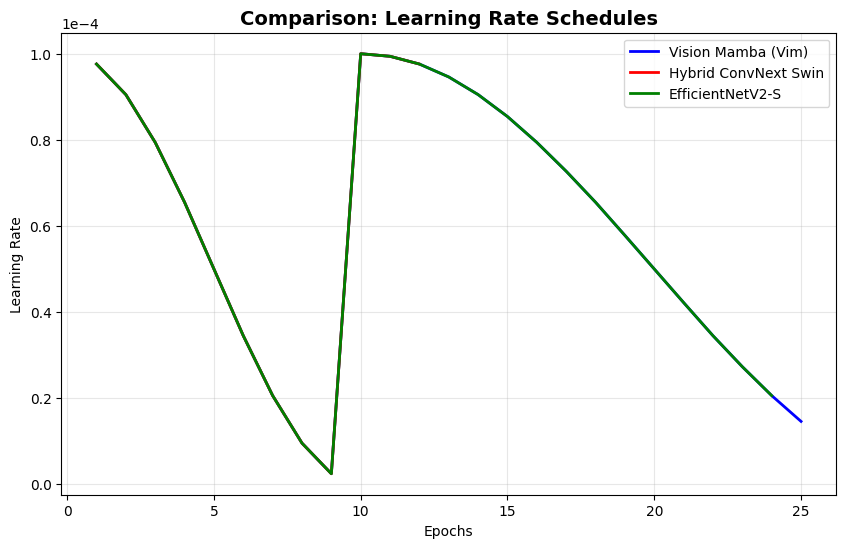
\includegraphics[width=\columnwidth]
{figures/learning_rate_curve.png}}
\caption{Learning rate scheduling curves across training epochs utilizing CosineAnnealingWarmRestarts for optimal model convergence.}
\label{fig:learning_rate_curve}
\end{figure}

\subsection{Robustness Under Gaussian Noise}

Table~\ref{tab:robustness} presents robustness 
evaluation results. A clear performance hierarchy 
emerges under increasing noise.

\begin{table}[htbp]
\caption{Robustness Evaluation Under Gaussian Noise Perturbation}
\begin{center}
\resizebox{\columnwidth}{!}{%
\begin{tabular}{lcccccccc}
\toprule
\multirow{2}{*}{\textbf{Model}} & 
\multicolumn{2}{c}{$\boldsymbol{\sigma=0.00}$} & 
\multicolumn{2}{c}{$\boldsymbol{\sigma=0.05}$} & 
\multicolumn{2}{c}{$\boldsymbol{\sigma=0.10}$} & 
\multicolumn{2}{c}{$\boldsymbol{\sigma=0.20}$} \\
\cmidrule(lr){2-3}\cmidrule(lr){4-5}
\cmidrule(lr){6-7}\cmidrule(lr){8-9}
 & Acc & AUC & Acc & AUC & Acc & AUC & Acc & AUC \\
\midrule
Vim (M1) & 99.89 & 1.000 & 98.44 & 0.9997 & 
95.44 & 0.9928 & 82.78 & 0.9123 \\
Conv+Swin (M2) & 99.67 & 1.000 & \textbf{99.78} & 
\textbf{1.000} & \textbf{93.00} & \textbf{0.9946} & 
\textbf{83.22} & \textbf{0.9444} \\
EfficientV2 (M3) & 99.33 & 0.9999 & 90.33 & 
0.9783 & 72.22 & 0.8918 & 56.56 & 0.7781 \\
\bottomrule
\multicolumn{9}{l}{\small Accuracy (\%); AUC-ROC (0--1 scale).}
\end{tabular}%
}
\label{tab:robustness}
\end{center}
\end{table}

The ConvNeXt-Swin hybrid demonstrates the highest 
noise resilience overall, achieving 99.78\% accuracy 
at $\sigma=0.05$ (marginally exceeding its clean 
accuracy, suggesting slight beneficial regularization 
effect from low-level noise). At $\sigma=0.20$, 
M2 retains 83.22\% accuracy and 0.9444 AUC, 
significantly outperforming M3. Vision Mamba 
exhibits intermediate robustness, maintaining 
95.44\% at $\sigma=0.10$ before declining to 
82.78\% at $\sigma=0.20$. EfficientNetV2 shows 
the sharpest degradation, dropping to 56.56\% 
accuracy at $\sigma=0.20$, approaching chance 
level, indicating that MSFA features are 
sensitive to high-frequency noise corruption. 
These findings suggest that hybrid multi-branch 
architectures provide superior robustness compared 
to single-backbone designs.

\begin{figure*}[!t]
\centerline{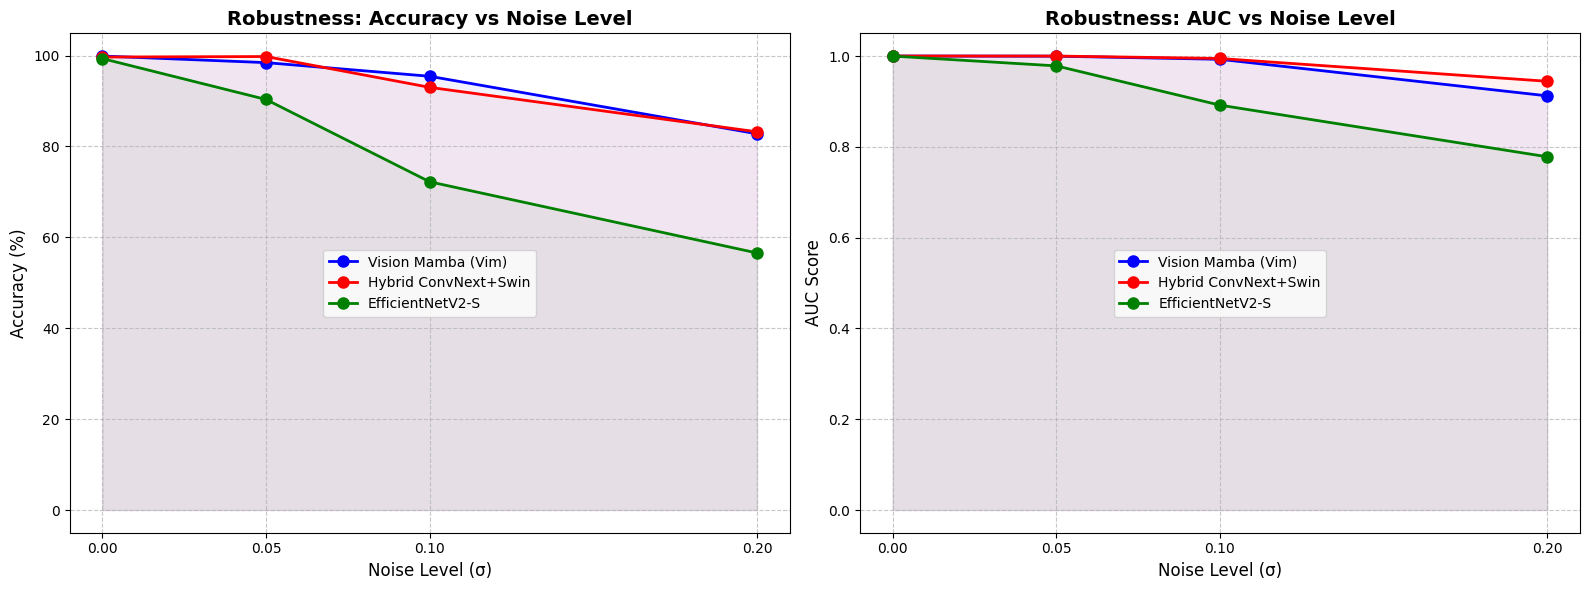
\includegraphics[width=\textwidth]
{figures/robustness.png}}
\caption{Robustness comparison: accuracy vs. 
Gaussian noise level ($\sigma$) for all three models. 
The ConvNeXt-Swin hybrid (M2) demonstrates 
superior noise resilience across all perturbation levels. The figure is enlarged for a detailed view of the performance trajectories.}
\label{fig:robustness}
\end{figure*}

\subsection{Explainability Analysis}

Fig.~\ref{fig:gradcam} presents representative 
Grad-CAM visualizations for correctly classified 
glaucomatous and normal fundus images. All three 
models concentrate activation in the optic disc 
region, consistent with established clinical 
diagnostic criteria focusing on cup-to-disc ratio, 
rim thinning, and disc hemorrhage. Vision Mamba 
produces spatially diffuse activations reflecting 
its sequence-based global feature integration, 
while the ConvNeXt-Swin hybrid generates sharper, 
more localized attention maps attributable to 
its dual-branch spatial attention architecture. 
EfficientNetV2 CBAM attention maps further 
highlight neuroretinal rim regions, demonstrating 
that channel attention selectively amplifies 
pathologically relevant feature channels.

\begin{figure*}[!t]
\centerline{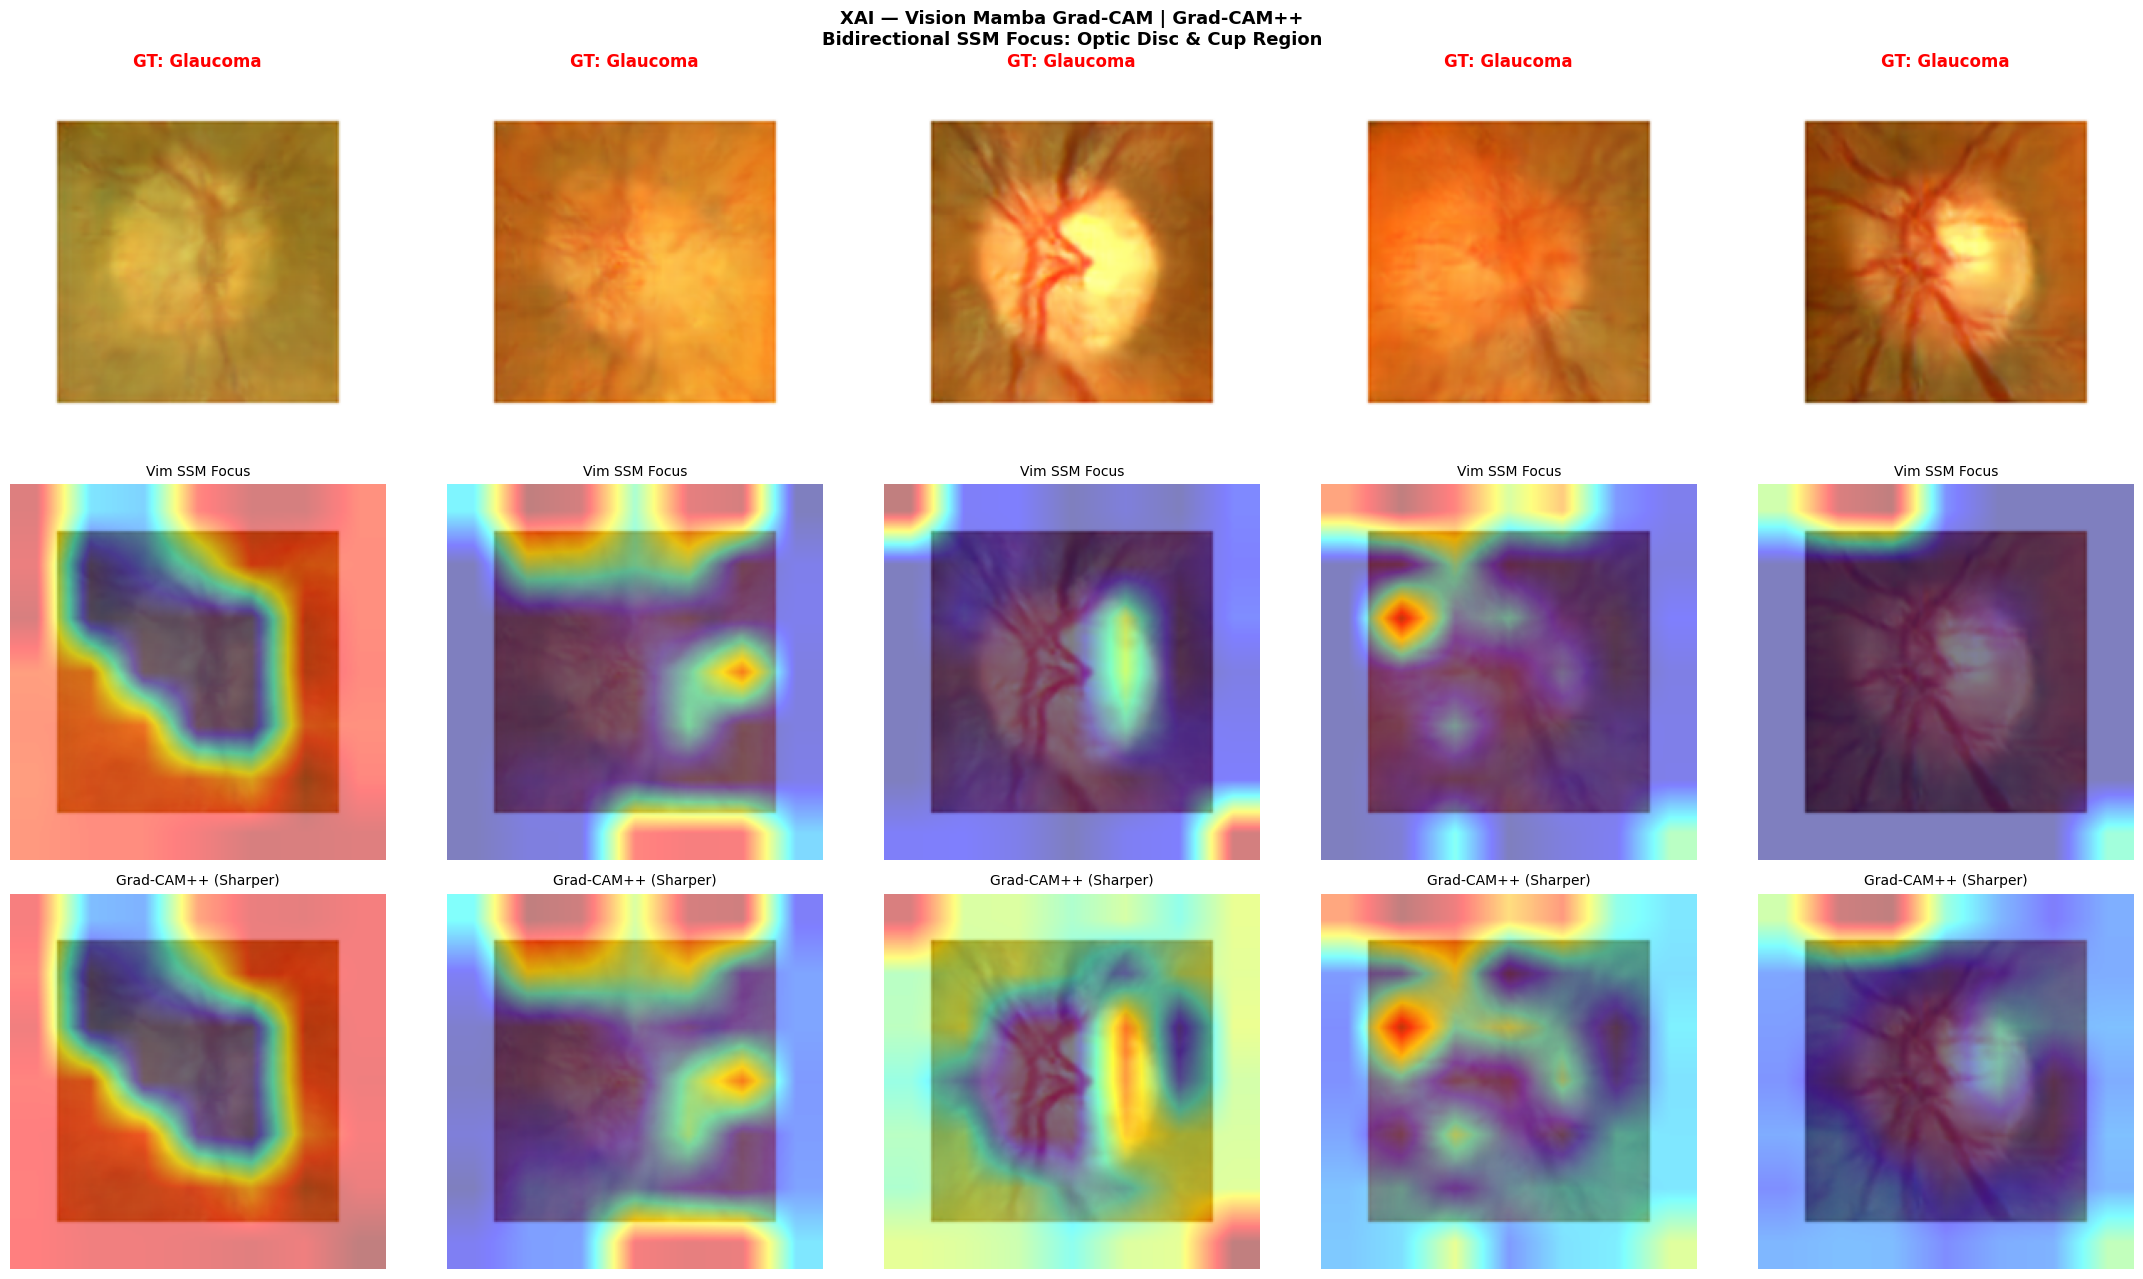
\includegraphics[width=\textwidth]
{figures/xai_grad_cam.png}}
\caption{Grad-CAM visualizations for glaucoma 
(top row) and normal (bottom row) cases across 
M1 (Vim), M2 (ConvNeXt+Swin), and M3 
(EfficientNetV2). Warmer colors indicate higher 
activation. All models correctly localize 
attention to the optic disc region, presented in a two-column layout for enhanced interpretability.}
\label{fig:gradcam}
\end{figure*}

\subsection{Comparative Analysis with Literature}

Table~\ref{tab:sota} contextualizes our results 
against recent glaucoma detection literature. 
Our Vision Mamba model achieves a new 
state-of-the-art on the ACRIMA dataset, 
while all three proposed architectures 
collectively advance performance benchmarks 
for binary glaucoma classification from fundus images.

\begin{table}[htbp]
\caption{Comparison with State-of-the-Art Methods on ACRIMA}
\begin{center}
\begin{tabular}{llcc}
\toprule
\textbf{Reference} & \textbf{Architecture} & 
\textbf{Acc. (\%)} & \textbf{AUC} \\
\midrule
Diaz-Pinto et al. \cite{b8}   & ResNet-50       & 93.70 & 0.971 \\
Bajwa et al. \cite{b9}         & DenseNet-121    & 96.30 & 0.982 \\
Li et al. \cite{b10}           & EfficientNet-B4 & 97.80 & 0.991 \\
Khan et al. \cite{b11}         & Swin-B          & 98.50 & 0.995 \\
\midrule
\textbf{Ours (M3 Effv2)} & EfficientV2+CBAM+GeM & 99.33 & 0.9999 \\
\textbf{Ours (M2 Hybrid)}& ConvNeXt+Swin+CBAM   & 99.67 & 1.0000 \\
\textbf{Ours (M1 Vim)}   & Vision Mamba V3       & \textbf{99.89} & \textbf{1.0000} \\
\bottomrule
\end{tabular}
\label{tab:sota}
\end{center}
\end{table}




%=============================================================
%  SECTION VII — CONCLUSION
%=============================================================
\section{Conclusion}
\label{sec:conclusion}

This paper presented a comprehensive comparative 
evaluation of three advanced deep learning 
architectures for automated glaucoma detection 
from color fundus photographs using the ACRIMA 
dataset. Vision Mamba (Vim) achieved the 
highest classification accuracy of 99.89\% 
with a perfect AUC-ROC of 1.0000, establishing 
a new benchmark for glaucoma classification 
from fundus images. The hybrid ConvNeXt-Swin 
architecture demonstrated superior robustness 
under Gaussian noise perturbation, maintaining 
99.78\% accuracy even at moderate noise levels, 
making it the preferred choice for real-world 
clinical deployment scenarios. EfficientNetV2-S 
with MSFA augmentation offered the most 
parameter-efficient solution at 20.9M parameters, 
suitable for resource-constrained deployment.

Explainability analysis via Grad-CAM confirmed 
that all models correctly focus on the optic 
disc and cup region, consistent with 
ophthalmological diagnostic criteria. 
Temperature scaling calibration on the 
ConvNeXt-Swin hybrid further enhances 
probabilistic reliability for clinical 
risk-stratified referral systems.

Future work will extend evaluation to 
multi-dataset cross-validation, incorporate 
optic disc segmentation as an auxiliary task, 
and explore federated learning frameworks 
for privacy-preserving multi-center clinical 
deployment. Integration of optical coherence 
tomography (OCT) data with fundus images 
in a multi-modal fusion framework represents 
a particularly promising research direction.


%=============================================================
%  ACKNOWLEDGMENT
%=============================================================
\section*{Acknowledgment}

The authors thank [Institution/Lab Name] for 
providing computational resources. This work 
was supported by [Funding Agency and Grant Number].


%=============================================================
%  REFERENCES
%=============================================================
\bibliographystyle{IEEEtran}
\bibliography{rf}

\end{document}